\subsection{Memento (\textit{o Token})}
\label{memento}

\textbf{Scopo}: Comportamentale \\
\textbf{Raggio d'azione}: Oggetti

\paragraph{Definizione} Il pattern, senza violare l'incapsulamento, cattura ed esternalizza lo stato interno di un oggetto in modo che l'oggetto possa essere ripristinato a questo stato in un secondo momento.

\paragraph{Motivazione} A volte è necessario registrare lo stato interno di un oggetto, cosa richiesta quando si implementano checkpoint e meccanismi di undo che permettono agli utenti di annullare operazioni tentative o recuperare da errori. Devi salvare informazioni di stato da qualche parte per poter ripristinare gli oggetti ai loro stati precedenti, ma gli oggetti normalmente incapsulano parte o tutto il loro stato, rendendolo inaccessibile ad altri oggetti e impossibile da salvare esternamente, e esporre questo stato violerebbe l'incapsulamento, compromettendo l'affidabilità e l'estensibilità dell'applicazione. Considera per esempio un editor grafico che supporta la connettività tra oggetti dove un utente può connettere due rettangoli con una linea e i rettangoli rimangono connessi quando l'utente muove uno di essi, con l'editor che assicura che la linea si estenda per mantenere la connessione. 

\begin{multicols}{2}
    \begin{figure}[H]
        \centering
        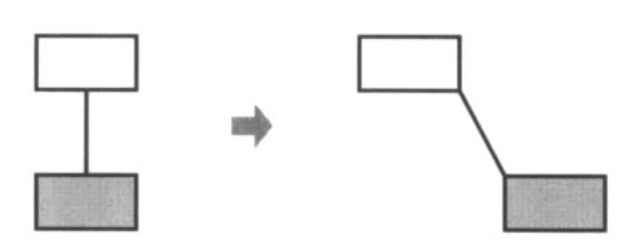
\includegraphics[width=1\linewidth]{assets/pattern/memento/memento-esempio-1.png}
    \end{figure}
    \columnbreak
    \vline
    \begin{figure}[H]
        \centering
        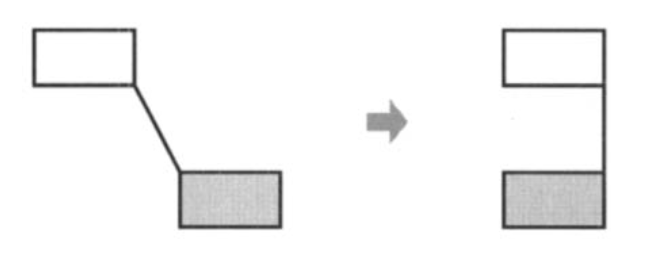
\includegraphics[width=1\linewidth]{assets/pattern/memento/memento-esempio-2.png}
    \end{figure}
\end{multicols}

Un modo noto per mantenere relazioni di connettività tra oggetti è con un sistema di risoluzione di vincoli incapsulato in un oggetto ConstraintSolver che registra le connessioni mentre vengono fatte e genera equazioni matematiche che le descrivono. Supportare l'undo in questa applicazione non è facile come può sembrare: un modo ovvio per annullare un'operazione di movimento è memorizzare la distanza originale spostata e muovere l'oggetto indietro di una distanza equivalente, tuttavia questo non garantisce che tutti gli oggetti appariranno dove erano prima. In generale, l'interfaccia pubblica del ConstraintSolver potrebbe essere insufficiente per permettere l'inversione precisa dei suoi effetti su altri oggetti, e il meccanismo di undo deve lavorare più strettamente con ConstraintSolver per ristabilire lo stato precedente, ma dovremmo anche evitare di esporre gli interni del ConstraintSolver al meccanismo di undo. Possiamo risolvere questo problema con il pattern Memento: un memento è un oggetto che memorizza un'istantanea dello stato interno di un altro oggetto—l'originatore del memento—dove il meccanismo di undo richiederà un memento dall'originatore quando deve fare un checkpoint dello stato dell'originatore, e l'originatore inizializza il memento con informazioni che caratterizzano il suo stato corrente, dove solo l'originatore può memorizzare e recuperare informazioni dal memento poiché il memento è "opaco" ad altri oggetti.

\newpage

\paragraph{Applicabilità} È opportuno usare il pattern Memento quando:
\begin{itemize}
    \item Si deve memorizzare un'istantanea (totale o parziale) dello stato di un oggetto, così da poterla ripristinare in un secondo tempo;
    \item Si vogliono proteggere dettagli implementativi che violerebbero l'incapsulamento.
\end{itemize}

\begin{figure}[H]
    \centering
    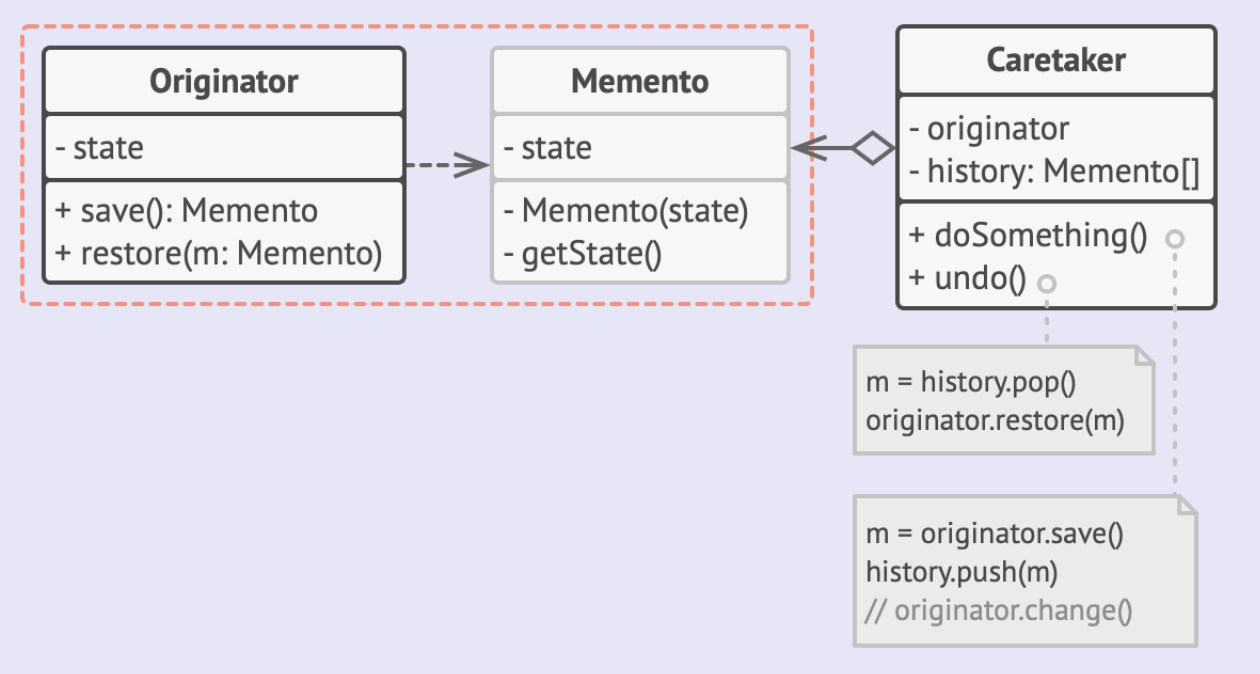
\includegraphics[width=1\linewidth]{assets/pattern/memento/memento-struttura.png}
    \caption{Class Diagram del pattern Memento}
\end{figure}

\paragraph{Struttura} Il pattern è composto da
\begin{itemize}
    \item \textbf{Memento}: memorizza lo stato interno dell’oggetto Originator, non permette l’accesso alla sua struttura dati se non all’Originator, presentando così due interfacce.
    \item \textbf{Originator} Crea un Memento contenente un’istantanea del proprio stato interno corrente. Usa un Memento per ripristinare il proprio stato interno tramite l’interfaccia estesa di Memento, con la quale è possibile accedere a tutti i dati necessari. Idealmente solo l’Originator che ha prodotto il Memento ha il permesso di accedere allo stato interno del Memento. 
    \item \textbf{Caretaker} È responsabile di memorizzare i Memento. Non invoca operazioni né esamina i contenuti di un Memento, vede un’interfaccia ridotta di Memento e può solo passare il Memento ad altri oggetti.
\end{itemize}

In altre implementazioni, la classe Memento è annidata all'interno di Originator. Ciò consente all'Originator di accedere ai campi e ai metodi del Memento, anche se sono dichiarati privati. D'altra parte, il Caretaker ha un accesso molto limitato ai campi e ai metodi del ricordo, il che gli consente di archiviare i ricordi in uno Stack ma di non manometterne lo stato.

\paragraph{Conseguenze} Il pattern Mediator consente quindi di:
\begin{itemize}
    \item Preservare i confini dell'incapsulamento
    \item Semplificare l'Originator
    \item Definire interfacce \textit{narrow and wide}
\end{itemize}

È bene notare che l'uso dei Memento potrebbe essere costoso, esistono dei costi nascosti (soprattutto in termini di memoria, ma anche di gestione).

\begin{figure}[H]
    \centering
    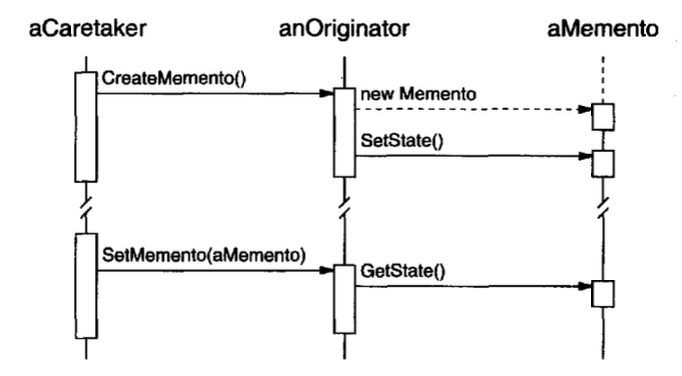
\includegraphics[width=0.75\linewidth]{assets/pattern/memento/memento-sequence.png}
    \caption{Sequence Diagram del pattern Memento}
\end{figure}

\newpage